\documentclass[12pt, a4paper]{article}
\usepackage[utf8]{inputenc}
\usepackage[brazil]{babel}
\usepackage{graphicx} \graphicspath{ {../img/} }
\usepackage{hyperref}
\usepackage{abnt-alf}
\usepackage[top=3cm,bottom=2cm,left=3cm,right=2cm]{geometry}
\usepackage{indentfirst}
\usepackage[table,xcdraw]{xcolor}
\usepackage{subfigure}
\usepackage{amsmath}
\usepackage{import}

% O tamanho do parágrafo é dado por:
\setlength{\parindent}{1.3cm}

% Controle do espaçamento entre um parágrafo e outro:
\setlength{\parskip}{0.2cm}  % tente também \onelineskip
% Retira espaço extra obsoleto entre as frases.
\frenchspacing 

\title{A operação de diferença entre templates de autômatos celulares}
\author{Zorandir Soares Junior \footnote{zorandir@gmail.com} \\
 	Programa de Pós-Graduação em Engenharia Elétrica e Computação \\
	Universidade Presbiteriana Mackenzie
	\and
	Pedro Paulo Balbi de Oliveira \footnote{pedrob@mackenzie.br}  \\
 	Programa de Pós-Graduação em Engenharia Elétrica e Computação \\
	Universidade Presbiteriana Mackenzie
	}

\date{\today} 

\begin{document}
\citeoption{abnt-etal-cite=3}
\citeoption{abnt-etal-list=5}
\citeoption{abnt-etal-text=3}

% DESENVOLVIMENTO
\pagestyle{plain}
\renewcommand{\baselinestretch}{1.25} 
\normalsize

\maketitle

\begin{abstract}
 Este artigo apresenta a operação de diferença entre templates e sua aplicabilidade. Para isto introduz o que são templates e como o uso de templates pode ajudar na representação de famílias de autômatos celulares. Apresenta também algumas operações aplicáveis aos templates, assim como introduz a operação que gera templates de exceção.

\begin{flushleft}
{\bf Palavras-chave:} {\it Autômatos celulares, espaço de regras, templates, diferença de templates, templates de exceção.}
\end{flushleft}
\end{abstract}

\section{INTRODUÇÃO}
\label{sec:introducao}
Autômatos celulares (ACs) são sistemas dinâmicos tipicamente discretos em tempo, espaço e estados \cite{wolfram2002}. Por meio de regras de ações locais simples os ACs têm a capacidade de gerar comportamentos globais complexos. O estudo de problemas clássicos de autômatos celulares, como o problema da paridade \cite{Betel2013} e o problema da densidade \cite{deOliveira2014density}, podem ajudar a compreender como esse comportamento complexo surge.

Há algumas maneiras de se buscar a solução para esses problemas clássicos, sendo a mais básica simplesmente testar todas as regras de uma determinada família de ACs afim de verificar se alguma dessas regras resolve o problema buscado. Entretanto, para grandes famílias de ACs, que é a situação mais usual, essa abordagem se mostra ineficiente, senão impraticável.

Como estratégia de pesquisa nessas famílias maiores, algoritmos de busca têm sido utilizados, em particular os de computação evolutiva, os quais já se mostraram muito eficazes no problema de classificação de densidade \cite{wolz2008very}.

Outra estratégia na busca de regras é a restrição do espaço de busca por regras que apresentem determinada propriedade. Para conseguir representar um subespaço com determinada propriedade sem a necessidade de se enumerar todas as regras nele contidas, pode-se utilizar a ideia de \textit{templates}, conforme proposta em \cite{deOliveira2014,deOliveira2014b}.

Há uma série de operações que podem ser aplicadas aos templates, como expansão e intersecção. No presente artigo é introduzida a operação de \textit{diferença entre templates} e a operação geradora de \textit{templates de exceção}. Além disso são mostrados alguns exemplos de aplicação dessas operações.

Depois de a próxima seção apresentar algumas noções básicas sobre autômatos celulares, a Seção \ref{sec:templates}
 apresenta em mais detalhes o que são templates e suas principais operações. A Seção \ref{sec:diferenca_entre_templates_e_templates_de_excecao}
 introduz as operações de diferença entre templates e de geração de templates de exceção, assim como suas aplicações. Por fim, a Seção \ref{sec:consideracoes_finais} faz considerações finais sobre as novas operações e menciona trabalhos futuros.

\section{Autômatos Celulares}
\label{sec:automatos_celulares}
Autômatos celulares são idealizações matemáticas simples dos sistemas naturais \cite{wolfram1994cellular}. Eles consistem em um reticulado de campos discretos usualmente idênticos, chamados de células, onde cada uma pode assumir um conjunto finito de, geralmente, valores inteiros. Os valores (ou estados) das células evoluem em tempo discreto de acordo com regras usualmente determinísticas que especificam o estado de cada célula de acordo com os estados de suas células vizinhanças \cite{wolfram1994cellular}.

Usualmente, assume-se que as células de um autômato celular apresentam $k$ estados, os quais são representados por valores inteiros no intervalo $[0, k-1]$. O estado de uma célula é modificado pela função local do autômato (sua regra), formada pelo conjunto de transições de estado de uma célula, baseado em seu estado atual e nos estados das células adjacentes. Para que as funções locais atualizem os valores de uma célula, usualmente um raio de ação $r$ é definido, o qual representa o número de células adjacentes que serão analisadas em cada direção pelas funções locais.

Uma família, ou espaço, de autômatos celulares é definida pelo raio $r$ e pelo número de estados $k$. Autômatos celulares unidimensionais de raio $r=1$ e $k=2$ são conhecidos como a família dos autômatos celulares elementares.

O número de regras de um espaço é dado por $k^{k^{2r+1}}$, tornando fácil perceber que qualquer modificação nas variáveis $k$ e $r$ geram famílias com um total de regras muito grande. Uma boa estratégia para lidar com esse problema é a utilização de propriedades estáticas, que são propriedades obtidas diretamente do conjunto de transições de estado do AC. Ao utilizar propriedades estáticas, pode-se restringir bastante o espaço de busca original. Com templates é possível representar um conjunto de regras com determinada propriedade estática.

Entretanto, para poder explicar o funcionamento dos templates e suas operações é interessante compreender os detalhes das propriedades de conservabilidade de estados, simetria interna e das regras invariantes a troca de cor, pois essas propriedades serão usadas como exemplo posteriormente.

\subsection{Conservabilidade de Estados}
Conservabilidade de estados é uma propriedade estática que determina que a soma dos estados de um determinado autômato celular não deve se alterar durante a evolução espaço-temporal, independente da configuração inicial.

De acordo com Boccara e Fukś (\citeyear{boccara2002}), um AC é conservativo quando cada uma de sua função local $f$, aplicada em cada vizinhança $(\alpha_0,\alpha_1, \dots, \alpha_{n-1})$ respeita as condições descritas na Eq. \eqref{eq:conservativeCA}.
\begin{equation}
\begin{split}
f(\alpha_0,\alpha_1, \dots,\alpha_{n-1}) = \alpha_0 + (\sum_{i=0}^{n-2}f(0_0,0_1, \dots,0_i,\alpha_1,\alpha_2, \dots,\alpha_{n-1}) \\- f(0_0,0_1, \dots,0_i,\alpha_0,\alpha_1, \dots,\alpha_{n-i-1}))
\label{eq:conservativeCA}
\end{split}
\end{equation}

\subsection{Simetria Interna}
Para compreender a propriedade de simetria interna, é necessário primeiro introduzir a noção de equivalência dinâmica entre regras. As explicações a seguir são válidas para regras binárias, apesar de ser possível sua generalização para $k$ estados.

Dada a tabela de transições de um AC, existem três transformações que podem ser empregadas e que resultam em ACs com comportamentos dinâmicos equivalentes: \textit{reflexão}, \textit{conjugação} e \textit{composição}. A reflexão é a transformação obtida ao refletir os bits das vizinhanças da tabela de transições. A conjugação é obtida ao inverter todos os estados das células da tabela de transições. Já a composição é a transformação obtida ao se efetuar a reflexão e a conjugação, independente da ordem.

Para exemplificar essas transformações e as equivalências dinâmicas considere-se a tabela de transição da regra 60 do espaço elementar, conforme ilustra a Figura \ref{fig:table60}. Ao se aplicar a transformação por reflexão na regra 60 obtemos a regra 102 do espaço elementar, ilustrada pela Figura \ref{fig:table102}.

	\begin{figure}[h!]
	  \centering
	  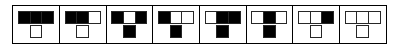
\includegraphics[width=.5\textwidth]{fig_ruleIcon60.png}
	  \caption{Tabela de transições da regra 60 do espaço elementar.}
	  \label{fig:table60}
	\end{figure}

	\begin{figure}[h!]
	  \centering
	  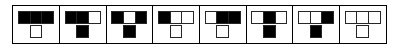
\includegraphics[width=.5\textwidth]{fig_ruleIcon102.png}
	  \caption{Tabela de transições da regra 102 do espaço elementar, obtida através da transformação de reflexão aplicada na tabela de transições da regra 60.}
	  \label{fig:table102}
	\end{figure}

% Tanto a regra 60, como as regras 102, 153 e 195 pertencem a mesma classe de equivalência dinâmica. Uma forma interessante de entender o porquê é analisando a evolução espaço-temporal dessas regras, ilustrada pela Figura \ref{fig:dynamicEquivalecy}.

% 	\begin{figure}[h!]
% 	  \centering
% 	  \def\svgscale{0.45}
% 	  \import{../img/}{fig_ruleEquivalence60.pdf_tex}
% 	  \caption{Evolução espaço-temporal das regras pertencente à mesma classe dinâmica da regra 60.}
% 	  \label{fig:dynamicEquivalecy}
% 	\end{figure}

A simetria interna é definida pela quantidade de transições de estado que permanecem iguais após aplicada uma determinada transformação. Exemplificando, a regra 60 dos ACs elementares tem um valor de simetria interna por reflexão igual a 4, pois compartilha as transições de estado $((1,1,1),0)$, $((1,0,1),1)$, $((0,1,0),1)$ e $ ((0,0,0),0)$ com a regra resultante de sua transformação por reflexão, a regra 102.

\subsection{Invariância a troca de cor}
Considera-se que um AC tem a propriedade de invariância a troca de cor se ele for invariante à aplicação de permutações nos estados das células de sua tabela de transição \cite{salo2013color}. Naturalmente, em geral há $k!$ permutações possíveis, mas no caso binário apenas uma, que pode ser descrita como $\{0 \to 1 ,\, 1 \to 0\}$. 

A propriedade de invariância a troca de cores está diretamente ligada à transformação por conjugação, sendo que as regras invariantes a troca de cor são as regras que possuem máxima simetria interna por conjugação.

\section{Templates}
\label{sec:templates}
Template é uma generalização das tabelas de transições de estado de ACs por meio de variáveis. Um único template pode representar um conjunto de regras que podem apresentar determinada propriedade. Os templates foram criados e implementados por De Oliveira e Verardo (\citeyear{deOliveira2014}) e são atualmente disponíveis na biblioteca \textit{open source CATemplates} \cite{CATemplates} no GitHub.

Formalmente, um \textit{template} é uma $n$-upla formada por $k^{2r+1}$ itens, em que cada item $i$ representa uma função $g_i(x_0,x_1,\dots,x_{k^{2r+1}-1})$. As variáveis $x_i$ podem assumir qualquer estado entre 0 e $k-1$. É possível limitar os valores possíveis de $x_i$ através da notação $x_i \in C$, onde $C$ é um conjunto representando os possíveis valores de $x_i$. %TODO verificar essa função $g_i$

Exemplificando, o template do espaço elementar $T_1 = (1,1,1,1,1-x_1,x_2,x_1,0)$ representa todas as regras que tenham na posição 0 (sempre da direita pra esquerda) o estado 0, nas posições 4, 5, 6 e 7 o estado 1, nas posições 1 e 2 qualquer estado no intervalo $[0,k-1]$ e na posição 3 o estado complementar ao valor da posição 1. Deste modo o template $T_1$ representa o conjunto de autômatos celulares elementares $\{(1,1,1,1,1,0,0,0),(1,1,1,1,0,0,1,0),(1,1,1,1,1,1,0,0),(1,1,1,1,0,1,1,0)\}$, ou em sua forma decimal $\{248,242,252,246\}$. O processo de encontrar todas as regras representadas por um template se chama \textit{expansão}.

Já há implementado na biblioteca \textit{CATemplates} \cite{CATemplates} diversos algoritmos geradores de templates que representem regras com determinada propriedade. O template $T_{comp} = (1 - x_0, 1 - x_4, 1 - x_2, x_4, 1 - x_1, x_2, x_1, x_0)$ dos ACs elementares, por exemplo, quando expandido gera apenas regras que apresentam máxima simetria interna por composição. Já o template $T_{inv} = (1 - x_0, 1 - x_1, 1 - x_2, 1 - x_3, x_3, x_2, x_1, x_0)$ dos AC elementares se expande apenas nas regras com propriedade de invariância a troca de cor.

Além da possibilidade de expansão de templates, já foi desenvolvido por De Oliveira e Verardo (\citeyear{deOliveira2014b}) um algoritmo que permite gerar templates que representem a intersecção entre dois sub-espaços de regras representadas por templates. Para exemplificar, considere-se a busca por um conjunto de regras que sejam ao mesmo tempo invariantes a troca de cor e apresentem máxima simetria interna por composição. Para encontrar esse conjunto de regras basta realizar dois passos.

O primeiro passo é igualar os dois templates que representam as propriedades desejadas, gerando assim um sistema de equações. Ao solucionar esse sistema de equações serão gerados os relacionamentos entre as variáveis, que quando aplicados aos templates recebidos como entrada, resultará no template que representa a intersecção.

Como exemplo, seja o template $T_{comp}$, que representa as regras com máxima simetria por composição, e o template $T_{inv}$, que representa as regras invariantes a troca de cor, ambos com $k=2$ e $r=1$. O primeiro passo para encontrar a intersecção entre esses dois template consiste em igualá-los gerando o sistema de equações representado pela Eq. \ref{eq:interseccaoP1}:
\begin{equation}
\left\{\begin{matrix}
1 - x_0	& = & 1 - x_0	\\
1 - x_4	& = & 1 - x_1	\\
1 - x_2	& = & 1 - x_2	\\
x_4		& = & 1 - x_3	\\
1 - x_1	& = & x_3		\\
x_2		& = & x_2		\\
x_1		& = & x_1		\\
x_0		& = & x_0		\\
\end{matrix}\right.
\label{eq:interseccaoP1}
\end{equation}

Em seguida o sistema é resolvido, obtendo-se o conjunto solução $S = \{x_3 = 1-x1, x_4 = x_1\}$. Esse conjunto solução é então aplicado como um conjunto se substituições aos templates recebidos como parâmetro. Caso os templates recebidos como parâmetro não apresentem restrições de variáveis, o resultado de ambas as substituições podem ser escolhidos, finalizando o processo e resultando no template $(1 - x_0, 1 - x_1, 1 - x_2, x_1, 1 - x_1, x_2, x_1, x_0)$, o qual representa a intersecção dos templates $T_{comp}$ e $T_{inv}$ e, por consequência, todos as regras do espaço elementar que, ao mesmo tempo, são invariantes a troca de cor e têm máxima simetria por composição.

Caso pelo menos um dos templates apresente restrições de variáveis, uma segunda etapa deve ser realizada. Para tanto, as expressões que restringem as variáveis são extraídas, gerando um conjunto que é então traduzido para um novo sistema de equações a ser resolvido, cujo conjunto solução é então aplicado como um conjunto de substituições nos templates passados como parâmetro.

Inspirada na operação de intersecção, introduzimos neste artigo a operação de diferença entre templates.

\section{Diferença entre templates e Templates de Exceção}
\label{sec:diferenca_entre_templates_e_templates_de_excecao}

A operação de diferença recebe dois templates como parâmetro, que chamaremos de $T_{minuendo}$ e $T_{subtraendo}$. Essa operação tem como resultado um conjunto de templates que representa todas as regras representadas pelo template $T_{minuendo}$ que não são representadas também pelo $T_{subtraendo}$.

A operação de diferença é um processo com diversas etapas. A primeira delas consiste em fazer a intersecção entre os dois templates passados como parâmetro, resultando num template $T_i$. Caso não haja intersecção entre os dois templates originais, o resultado da diferença é o próprio $T_{minuendo}$. Caso haja intersecção, o template de intersecção $T_i$ é igualado ao template $T_{minuendo}$, gerando assim combinações lógicas de equações. Então o algoritmo remove as equações tautológicas e aplica uma operação de negação nas equação, que no caso binário consiste em apenas efetuar as permutações $\rho = (0 \to 1, 1 \to 0)$ ao resultado final das equações. Neste momento, deve-se trocar o operador lógico $\wedge$ por $\vee$ e o sistema gerado por esse processo é solucionado, gerando assim um conjunto de conjuntos de substituição que devem ser aplicados ao template $T_{minuendo}$. Caso o conjunto de substituições seja vazio ou inválido (i.e., que referenciam regras não existentes no espaço em questão, como exemplificado à frente), todas as regras que pertencem a $T_{minuendo}$ também pertencem ao $T_{subtraendo}$ e, por consequência, o algoritmo retorna um conjunto vazio.

Para melhor compreender o processo, considerem-se o template que representa as regras invariantes a troca de cor $T_{inv} = (1 - x_0, 1 - x_1, 1 - x_2, 1 - x_3, x_3, x_2, x_1, x_0)$ e o template de conservabilidade de estados $T_{con} = (1, 1 + x_2 - x_3, 1 - x_2, 1 - x_1 - x_2, x_3, x_2, x_1, 0)$, novamente ambos do espaço elementar. O primeiro passo para encontrar a diferença de $T_{inv}$ para $T_{con}$ é fazer a intersecção entre ambos, que resulta em $T_{int} = (1, 1 - x_1, 1 - x_2, 1 - x_1 - x_2, x_1 + x_2, x_2, x_1, 0)$. Como a intersecção é não nula, o próximo passo é igualar $T_{inv}$ com $T_{int}$, o que gera o sistema de equações representado pela Eq. \ref{eq:differenceP1}: \begin{equation} \left\{\begin{matrix} 1 - x_0	& = &	1				\\ 1 - x_1	& = &	1 - x_1			\\ 1 - x_2	& = &	1 - x_2			\\ 1 - x_3	& = &	1 - x_1 - x_2	\\
x_3		& = &	x_1 + x_2		\\
x_2		& = &	x_2				\\
x_1		& = &	x_1				\\
x_0		& = &	0				\\
\end{matrix}\right.
\label{eq:differenceP1}
\end{equation}

Entretanto, esse sistema deve ser representado por meio de combinações lógicas de equações, como se pode ver na Eq. \ref{eq:differenceP2}:
\begin{equation}
\begin{split}
1 - x_0	= 1				\wedge
1 - x_1	= 1 - x_1		\wedge
1 - x_2	= 1 - x_2		\wedge\\
1 - x_3	= 1 - x_1 - x_2	\wedge 
x_3		= x_1 + x_2		\wedge
x_2		= x_2			\wedge
x_1		= x_1			\wedge
x_0		= 0				
\label{eq:differenceP2}
\end{split}
\end{equation}

Eliminam-se então todas as equações tautológicas e trocam-se os operadores lógicos $\wedge$ por $\vee$, resultando no sistema representado pela Eq. \ref{eq:differenceP3}:
\begin{equation}
1 - x_0	= 1				\vee 
1 - x_3	= 1 - x_1 - x_2	\vee
x_3		= x_1 + x_2		\vee 
x_0		= 0				
\label{eq:differenceP3}
\end{equation}

Por fim, aplica-se a operação de negação nas equações que, no caso binário, corresponde à permutação $\rho $ ou,  de forma equivalente, à aplicação da função $f(x) = 1 - (x)$. A Eq. \eqref{eq:differenceP4} representa a combinação lógica de equações resultante dessas operações.
\begin{equation}
1 - x_0	= 1 - 1					\vee 
1 - x_3	= 1 - (1 - x_1 - x_2)	\vee
x_3		= 1 - (x_1 + x_2)		\vee 
x_0		= 1 - 0				
\label{eq:differenceP4}
\end{equation}

Resolve-se então a combinação lógica de equações, gerando o conjunto solução $S = \{\{x_0\to 1\},\{x_3\to -x_1-x_2+1\}\}$. Como $S$ apresenta mais de um conjunto de substituições, ambos os conjuntos devem ser utilizados para realizar as substituições no template $T_{inv} = (1 - x_0, 1 - x_1, 1 - x_2, 1 - x_3, x_3, x_2, x_1, x_0)$, obtendo-se finalmente o conjunto de templates $\{(0, 1 - x_1, 1 - x_2, 1 - x_3, x_3, x_2, x_1, 1),(1 - x_0, 1 - x_1, 1 - x_2, x_1 + x_2, 1 - x_1 - x_2, x_2, x_1, x_0)\}$

Em diversos casos apenas as etapas descritas até aqui são suficientes para se realizar a diferença entre os dois templates. Mas há casos em que o template $T_{subtraendo}$, correspondente a $T_{con}$ no exemplo dado, apresenta substituições nas variáveis que levam a regras inválidas. Tal situação ocorre, por exemplo, quando se expande o template $(1, 1 - x_1, 1 - x_2, 1 - x_1 - x_2, x_1 + x_2, x_2, x_1, 0)$ atribuindo-se o valor $1$ às variáveis $x_1$ e $x_2$. Aos se fazer isto será obtida na posição $3$ (da direita para esquerda) o valor $2$, que está fora do intervalo inteiro $[0,k-1]$, correspondendo, portanto, a uma regra que não faz parte do espaço tratado.

Para contornar esse problema, é necessário que, após os primeiros passos da operação de diferença, também se verifique se há templates de exceção na intersecção entre o $T_{minuendo}$ e o $T_{subtraendo}$, ou seja, templates que apresentam um conjunto de substituições que levam um template passado como parâmetro a apresentar substituições fora do intervalo $[0,k-1]$. %TODO melhorar esse texto

Exemplificando, vamos continuar a operação de diferença entre $T_{inv}$ e $T_{con}$; para tanto, seja o template $T_{int} = (1, 1 - x_1, 1 - x_2, 1 - x_1 - x_2, x_1 + x_2, x_2, x_1, 0)$ a intersecção entre eles, para $k=2$.
A primeira etapa da operação de diferença ocorre normalmente e gera os templates $\{(x_7, x_6, x_5, x_4, x_3, x_2, x_1, 1),(x_7, x_6, x_5, x_1 + x_2, x_3, x_2, x_1, x_0)\}$.
Mas é trivial perceber que qualquer expansão de $T_{int}$ que tenha o conjunto de substituições $\{x_1 = 1, x_2 = 1\}$ fará com que a posição $3$ e $4$ do template apresentem valores que não pertencem ao intervalo $[0,k-1]$.
Logo, todos os templates que apresentem $\{x_1 = 1, x_2 = 1\}$ são complementares ao template $T_{int}$. Assim gera-se o template $(x_7, x_6, x_5, x_4, x_3, 1, 1, x_0)$, que é o template de exceção de $T_{int}$.

Deste modo, toda regra representada pelo template $T_{minuendo}$ -- $T_{inv}$ no exemplo dado -- e que também seja representada pelos templates de exceção da intersecção do $T_{minuendo}$ com o $T_{subtraendo}$ -- $T_{int}$ no exemplo dado -- deve ser representada em algum dos templates resultantes da operação de diferença. Para tanto, o algoritmo que encontra a diferença entre templates considera todos os templates de exceção encontrados, intersecciona-os com o $T_{minuendo}$ e adiciona-os ao conjunto de templates obtidos pelos primeiros passos da operação de diferença. Com isso, no exemplo utilizado até agora, o conjunto de templates de diferença resultante está representado pela Eq. \ref{eq:differenceR}:\begin{equation}
\begin{split}
\{(0, 1 - x_1, 1 - x_2, 1 - x_3, x_3, x_2, x_1, 1), \\
(1 - x_0, 1 - x_1, 1 - x_2, x_1 + x_2, 1 - x_1 - x_2, x_2, x_1, x_0), \\
(1 - x_0, 0, 0, 1 - x_3, x_3, 1, 1, x_0)\}
\label{eq:differenceR}
\end{split}
\end{equation}

O interessante da operação de diferença entre templates é que com ela é possível descobrir respostas para diversas perguntas não triviais, como por exemplo, determinar quais são as regras que apresentam conservabilidade de estados, mas não apresentam ao mesmo tempo máxima simetria por composição nem invariância a troca de cor. Para responder a questão basta gerar o template de regras conservativas, e então subtrair dele a intersecção entre o template de regras com máxima simetria por composição e o template de invariância a troca de cor. Neste caso específico, o resultado é um conjunto de templates que representa todas as regras conservativas, excetuando a regra identidade.

Vale frisar que o conjunto de templates retornados não apresenta um espaço de busca menor do que template o $T_{minuendo}$; entretanto, a operação é capaz de representar a diferença entre dois templates sem a necessidade de se efetuar a expansão. Posteriormente os templates resultantes podem ser utilizados por outras operações, e essa é a principal vantagem da operação. 









\section{Considerações Finais}
\label{sec:consideracoes_finais}
No presente artigo são descritos os templates de autômatos celulares e apresentadas pela primeira vez a operação de diferença entre templates e a operação que encontra templates de exceção. Ambas as operações podem se mostrar valorosas em inúmeras situações que envolvam buscar uma regra num grande espaço, em particular nos clássicos problemas de paridade e de classificação densidade.

Mostra-se também como é possível obter resposta para perguntas não triviais sobre buscas por regras com determinadas propriedades estáticas, por meio de templates, sem depender da utilização de algoritmos de busca ou avaliações  enumerativas pro toda uma família de ACs.

Ressalte-se que a operação de diferença pode gerar um grande número de templates, o que pode, em casos específicos, não diminuir efetivamente o espaço de busca. Mas note-se que a abordagem é relevante em termos gerais e, tão mais efetiva quanto maior for a complexidade dos atributos especificados para as regras, ou seja, quanto maior for a quantidade de propriedades que o espaço de regras em questão deva ou não apresentar. Embora já fosse possível a especificação das propriedades desejadas pelos trabalhos anteriores de \cite{deOliveira2014,deOliveira2014b}%TODO Verificar citação
, com o presente trabalho passa a ser possível também a especificação das propriedades indesejadas.

Até o momento a operação de diferença entre templates foi implementada para as famílias de ACs com $k=2$, mas sua generalização para valores maiores de $k$ está em andamento.

\section*{Agradecimentos}
\label{sec:agrdecimentos}
Os autores agradecem ao Fundo Mackenzie de Pesquisa (MACKPESQUISA), à Fundação de Amparo à Pesquisa do Estado de São Paulo (FAPESP), e as agências federais CAPES e CNPq, por diferentes formas de apoio recebidos durante o desenvolvimento deste trabalho.

\def\refname{REFERÊNCIAS BIBLIOGRÁFICAS}
\bibliography{bibliografia}
\addcontentsline{toc}{section}{REFERÊNCIAS BIBLIOGRÁFICAS} 
\bibliographystyle{abnt-alf}

\end{document}